\section{Kreisel}
Im zweiten Teil des Experimentes wurde das Trägheitsmoment eines Kreisels bestimmt.
\subsection{Methoden}\label{kap:KreiselMethoden}
Zunächst wurde der Durchmesser der Kugel, die Länge l, die Masse m und für drei verschiedene Positionen des Zusatzgewichtes die Kraft F gemessen.
Jede dieser Messungen,bis auf die der Masse, wurde je 5 mal durchgeführt. Die Messergebnisse sind in Abb. \ref{fig:Kreisel} aufgeführt.
Die Längen  wurden mit einem Messschieber gemessen und die Masse mit einer Waage mit digitaler Anzeige.
\begin{figure}[h]
	\centering
	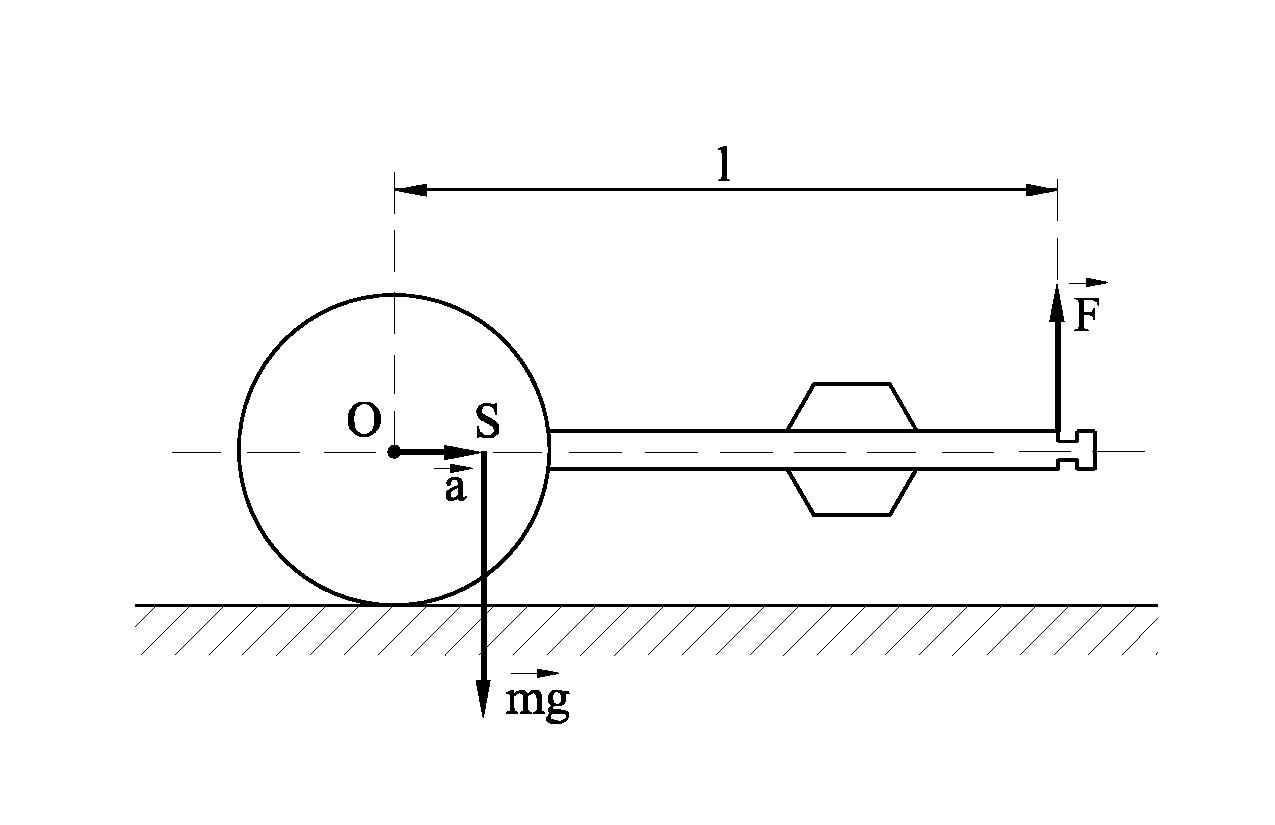
\includegraphics[width=\linewidth]{res/KreiselAufbau.pdf}
	\caption{Schematische Darstellung des Kreisels bei Messung der Kraft F\cite{lw}}
	\label{fig:kreisel}
\end{figure}
Mithilfe dieser Werte, dem aus der Anleitung gegeben Trägheitsmoment $J_{Stange}+J_{Zusatz}=\SI{15}{g \cdot cm^2}$ sowie den Formeln $J_{ges}=J_{Kugel}+J_{Stange}+J_{Zusatz}$ und $J_{Kugel}=\frac{2}{5}mr^2$ wurde der % in \cref{kap:Zusammenfassung} schon genannte
Wert für $J_{theo.}=\SI{1,3356+-0,0004e-4}{kg \cdot m^2}$ berechnet. Ein anderer Weg das Trägheitsmoment zu bestimmen war es, diesen über den Zusammenhang 
\begin{align}
2 \pi J= \frac{l \cdot F}{\frac{\Delta \omega}{\Delta T_p}} \label{eq:zusJlF}.
\end{align}
zu berechnen.
% zwischen l $\cdot$ F und  $\frac{\Delta \omega}{\Delta T_p}$ sowie dem Trägheitsmoment J.
Um dieses Verhältnis zu erhalten wurde die Präzessionszeit $T_p$ des Kreisels für drei unterschiedliche Positionen des Zusatzgewichtes bei fünf unterschiedlichen Frequenzen gemessen: Unten~(Position 1), mittig~(2) und oben~(3).Zur Messung der Frequenz des Kreisels wurde der Kreisel mit einem Stroboskop beleuchtet. Die Frequenz des Stroboskops wurde als erstes eingestellt anschließend wurde der Kreisel solange beschleunigt, bis er die gleiche Frequenz hatte, wie das Stroboskop.
Dass der Kreisel die gleiche Frequenz erreicht hatte, wie das Stroboskop wurde durch eine Markierung auf der Kugel des Kreisels ersichtlich. Sobald diese Markierung nahezu stillstand, war die Stroboskopfrequenz erreicht. Es war jedoch nicht möglich zu verhindern, dass sich diese Markierung weiterbewegte. Da die Markierung sich jedoch sowohl mit der Drehbewegung bewegte, als auch in die entgegengesetzte Richtung wurde bei den Rechnungen davon ausgegangen das sich diese entgegengesetzten Bewegungen in etwa aufheben. Die Präzessionzeit $T_p$ wurde gemessen indem der Kreisel leicht gekippt wurde und die Zeit für mehrere Umdrehungen der Stange gemessen wurde. Um die Winkelgeschwindigkeit $\omega$ zu erhalten wurde die Frequenz mit $2 \pi$ multipliziert.
Die Präzessionszeit wurde dann für jede Position des Zusatzgewichtes gegen die Winkelgeschwindigkeit aufgetragen. Die Messwerte wurde mit einem linearen Fit angepasst und das Produkt l $\cdot$ F wurde gegen den Kehrwert der drei Steigungen aufgetragen. Die Steigung der linearen Anpassung mit dem diese drei Punkte angepasst wurde entspricht $J \cdot 2 \pi$.